\section{Il modello di funzione logica con varianti}
\label{sec:variant-model}

Il supporto all'esecuzione energeticamente consapevole richiede che il 
sistema possa rappresentare, per una stessa funzione, implementazioni 
alternative con diversi profili di consumo e accuratezza. A tal fine è 
stato introdotto il concetto di \emph{funzione logica con varianti}: 
un'astrazione che raggruppa sotto un unico identificatore logico più 
implementazioni della stessa funzione, ciascuna caratterizzata da un 
proprio profilo energetico e da un modello di output che ne quantifica 
l'accuratezza.

\subsection{Struttura della funzione e profilo energetico}

In Serverledge, ogni funzione è rappresentata dalla struttura 
\texttt{Function}, estesa in questo lavoro con i campi necessari al 
supporto delle varianti energetiche. I campi rilevanti per il sistema 
proposto sono i seguenti:

\begin{itemize}
    \item \texttt{LogicalName}: identificatore condiviso da tutte le 
    varianti appartenenti alla stessa funzione logica. Costituisce 
    il riferimento con cui il client invoca la funzione, 
    indipendentemente dalla variante che verrà selezionata a runtime.

    \item \texttt{VariantID}: identificatore univoco della specifica 
    variante all'interno del gruppo logico (ad esempio \texttt{base}, 
    \texttt{light}, \texttt{c}).

    \item \texttt{EnergyProfile}: struttura che mantiene la stima 
    energetica della variante, composta da due campi:
    \begin{itemize}
        \item \texttt{ColdStartJoule}: energia stimata per l'avvio a 
        freddo del container, comprensiva dell'inizializzazione del 
        runtime;
        \item \texttt{InvocationJoule}: energia media stimata per una 
        singola invocazione della funzione
    \end{itemize}
    \item \texttt{AllowApprox}: flag booleano che indica se la funzione 
    logica ammette l'utilizzo di varianti approssimate. La sua 
    attivazione è condizione necessaria affinché lo scheduler 
    energy-aware possa considerare varianti con accuratezza ridotta.
\end{itemize}

\subsubsection{Determinazione dei profili energetici iniziali}

I valori iniziali di \texttt{EnergyProfile} sono stati determinati 
offline tramite una campagna di misurazioni preliminari condotta con 
Kepler. La metodologia adottata tiene conto della natura delle metriche 
esposte da Kepler: trattandosi di contatori cumulativi, l'energia 
osservata al termine di $n$ invocazioni consecutive sullo stesso 
container rappresenta la somma dei contributi di tutte le esecuzioni, 
inclusa quella iniziale soggetta al cold start.

Per separare i due contributi energetici si è proceduto nel modo 
seguente. Dato un container su cui vengono eseguite $n$ invocazioni 
consecutive, si indica con $E_{tot}$ l'energia cumulativa totale 
rilevata da Kepler al termine dell'ultima invocazione e con $E_1$ 
l'energia della prima invocazione, che comprende sia il costo di 
inizializzazione del container che quello di esecuzione della funzione. 
Le invocazioni successive, eseguite a container già attivo, sono invece 
soggette al solo costo di esecuzione. Il costo medio di invocazione in 
warm start è quindi stimato come:

\begin{equation}
    E_{inv} = \frac{E_{tot} - E_1}{n - 1}
    \label{eq:inv-joule}
\end{equation}

e il costo di cold start come:

\begin{equation}
    E_{cold} = E_1 - E_{inv}
    \label{eq:cold-joule}
\end{equation}

La ripetizione delle misurazioni su un numero statisticamente 
significativo di invocazioni consente di attenuare la varianza 
introdotta dal sistema operativo e dal runtime, ottenendo stime 
robuste per entrambi i contributi. I valori così ottenuti vengono 
codificati nel file JSON di definizione delle varianti e costituiscono 
la stima iniziale del profilo energetico. Il \autoref{lst:fibonacci-json} 
mostra un esempio concreto per la funzione \texttt{fibonacci}, che 
espone tre varianti con profili energetici distinti.

\begin{lstlisting}[
    language=json,
    caption={File di definizione delle varianti per la funzione 
    \texttt{fibonacci}. Ciascuna variante specifica runtime, entry 
    point, profilo energetico iniziale e modello di output.},
    label={lst:fibonacci-json}
]
{
  "variants": [
    {
      "id": "base",
      "runtime": "python310",
      "entry_point": "fibonacci.handler",
      "src": "fibonacci.py",
      "energy": {
        "cold_start_joule": 0.06606,
        "invocation_joule": 0.000731579
      },
      "output": { "type": "error", "error_estimate": 0.0 },
      "is_approximate": false
    },
    {
      "id": "optimization-py",
      "runtime": "python310",
      "entry_point": "fibonacci_o.handler",
      "src": "fibonacci_o.py",
      "energy": {
        "cold_start_joule": 0.05640,
        "invocation_joule": 0.000494737
      },
      "output": { "type": "error", "error_estimate": 0.0 },
      "is_approximate": false
    },
    {
      "id": "c",
      "runtime": "native",
      "entry_point": "fibonacci",
      "src": "fibonacci",
      "energy": {
        "cold_start_joule": 0.008268422,
        "invocation_joule": 0.000171579
      },
      "output": { "type": "error", "error_estimate": 0.0 },
      "is_approximate": false
    }
  ]
}
\end{lstlisting}

I valori iniziali del profilo energetico sono progressivamente 
raffinati a runtime dal worker periodico, che aggiorna entrambi i valori sulla base delle misurazioni effettive 
raccolte durante l'esecuzione in produzione. I risultati numerici 
delle misurazioni preliminari per tutte le varianti sono riportati 
nel Capitolo~\ref{cap:RisultatiSperimentali}.
\subsection{Il modello di output e la classificazione dell'accuratezza}
\label{sec:output-model}

Per consentire allo scheduler di confrontare le varianti in termini di 
accuratezza, ciascuna variante è dotata di un \texttt{OutputModel} che 
descrive la qualità del suo output. Il modello supporta due tipologie 
di classificazione, scelte in base alla natura computazionale della 
funzione:

\begin{itemize}
    \item \textbf{Tipo \texttt{error}}: adatto a funzioni il cui output 
    è un valore numerico misurabile. L'accuratezza è espressa tramite 
    il campo \texttt{error\_estimate}, che rappresenta l'errore relativo 
    atteso rispetto alla variante di riferimento. Una variante esatta 
    presenta \texttt{error\_estimate = 0.0}, mentre varianti approssimate 
    presentano valori positivi proporzionali alla deviazione introdotta 
    dalla semplificazione algoritmica adottata.

    \item \textbf{Tipo \texttt{quality}}: adatto a funzioni il cui 
    output non è facilmente quantificabile con un errore numerico, 
    come classificatori o modelli di machine learning. L'accuratezza 
    è espressa tramite un livello discreto: \texttt{high}, 
    \texttt{medium} o \texttt{low}, che riflette la qualità complessiva 
    del risultato prodotto dalla variante.
\end{itemize}

Il ~\autoref{lst:imageclassification-json} mostra un esempio 
applicativo del tipo \texttt{quality} per la funzione 
\texttt{ImageClassification}, in cui la variante base utilizza un 
modello di rete neurale più accurato ma più oneroso, mentre la 
variante \texttt{Light} adotta un modello più compatto a qualità ridotta.

\begin{lstlisting}[
    language=json,
    caption={File di definizione delle varianti per la funzione 
    \texttt{ImageClassification}. Il campo \texttt{quality} esprime 
    l'accuratezza in forma discreta, adatta a output non numericamente 
    quantificabili.},
    label={lst:imageclassification-json}
]
{
  "variants": [
    {
      "id": "base",
      "runtime": "python-ml",
      "entry_point": "ImageClassification.handler",
      "src": "ImageClassification.py",
      "energy": {
        "cold_start_joule": 1.894736842,
        "invocation_joule": 1.455263158
      },
      "output": { "type": "quality", "quality": "high" },
      "is_approximate": false
    },
    {
      "id": "Light",
      "runtime": "python-ml",
      "entry_point": "ImageClassificationLight.handler",
      "src": "ImageClassificationLight.py",
      "energy": {
        "cold_start_joule": 1.071052329,
        "invocation_joule": 0.22894768
      },
      "output": { "type": "quality", "quality": "low" },
      "is_approximate": true
    }
  ]
}
\end{lstlisting}

Lo scheduler converte internamente entrambe le rappresentazioni in un 
punteggio numerico (\emph{ErrorScore}) secondo una scala uniforme: 
per il tipo \texttt{error} viene utilizzato direttamente il valore di 
\texttt{error\_estimate}, mentre per il tipo \texttt{quality} i livelli 
\texttt{high}, \texttt{medium} e \texttt{low} vengono mappati 
rispettivamente a $0.0$, $1.0$ e $2.0$. La selezione privilegia 
sempre la variante con il punteggio più basso compatibile con il 
vincolo energetico, garantendo che la qualità del risultato sia 
massimizzata nei limiti imposti dalla richiesta.

La Tabella~\ref{tab:output-models} riassume il modello di output 
adottato per ciascuna delle funzioni utilizzate negli esperimenti.

\begin{table}[h]
    \centering
    \begin{tabular}{llll}
        \toprule
        \textbf{Funzione} & \textbf{Tipo} & 
        \textbf{Variante base} & \textbf{Variante approssimata} \\
        \midrule
        Fibonacci         & \texttt{error}   & 0.0  & 0.0 \\
        PiLeibniz         & \texttt{error}   & 0.0  & $1.99 \times 10^{-8}$ \\
        Sqrt              & \texttt{error}   & 0.0  & 0.043 \\
        VectorMagnitude   & \texttt{error}   & 0.0  & 0.04 \\
        SentimentAnalysis & \texttt{quality} & high & low \\
        ImageClassification & \texttt{quality} & high & low \\
        \bottomrule
    \end{tabular}
    \caption{Modello di output adottato per ciascuna funzione. Per il 
    tipo \texttt{error} il valore riportato è \texttt{error\_estimate}; 
    per il tipo \texttt{quality} il livello discreto assegnato.}
    \label{tab:output-models}
\end{table}
\subsection{Registrazione e indicizzazione delle varianti in etcd}
\label{sec:variant-registration}

Le varianti di una funzione logica vengono definite tramite un file 
JSON collocato nella directory \texttt{variants/<LogicalName>/} del 
progetto. Al momento della registrazione, il sistema legge questo file 
attraverso il componente \texttt{FileSource}, prepara il codice 
sorgente di ciascuna variante in formato tar e materializza le varianti 
in etcd attraverso la funzione \texttt{CreateInternalVariants}.

\subsubsection{Convenzione di denominazione}

La convenzione di denominazione distingue la variante di riferimento 
dalle varianti alternative. La prima variante definita nel file JSON, tipicamente quella a massima accuratezza, mantiene come nome interno 
esattamente il \texttt{LogicalName}, preservando la compatibilità con 
le invocazioni che non specificano alcuna preferenza energetica. Le 
varianti successive ricevono un nome composto nella forma 
\texttt{<LogicalName>-<VariantID>}. Per la funzione logica 
\texttt{fibonacci} (\autoref{lst:fibonacci-json}) ad esempio, i nomi interni assegnati sono:

\begin{itemize}
    \item \texttt{fibonacci} — variante base in Python
    \item \texttt{fibonacci-optimization-py} — variante ottimizzata 
    in Python
    \item \texttt{fibonacci-c} — variante compilata in C nativo
\end{itemize}

\subsubsection{Struttura delle chiavi in etcd}

Il sistema mantiene in etcd due livelli distinti di chiavi, ciascuno 
con una responsabilità specifica, come illustrato in 
Figura~\ref{fig:etcd-structure}.

Il primo livello, sotto il prefisso \texttt{/function/}, contiene una 
chiave per ogni variante registrata nel sistema, indipendentemente 
dalla funzione logica di appartenenza. Il valore associato è la 
serializzazione JSON completa della struttura \texttt{Function}, che 
include il runtime, il codice sorgente, il profilo energetico corrente 
e il modello di output. È su queste chiavi che il worker periodico 
scrive gli aggiornamenti del campo \texttt{InvocationJoule} ad ogni 
ciclo di raccolta.

Il secondo livello, sotto il prefisso 
\texttt{/index/logical/<LogicalName>/}, costituisce un indice che 
associa ciascun nome logico all'insieme delle sue varianti. La 
motivazione di questo indice è di natura prestazionale: poiché la 
selezione della variante avviene nel critical path della richiesta di 
invocazione, è necessario che lo scheduler possa recuperare 
rapidamente tutte le varianti di una funzione logica senza dover 
scorrere l'intero prefisso \texttt{/function/}, che contiene tutte 
le funzioni registrate nel sistema. Tramite l'indice, il recupero 
avviene con una singola query con prefisso su 
\texttt{/index/logical/<LogicalName>/}, restituendo esclusivamente le 
varianti della funzione richiesta e contenendo così la latenza 
introdotta dalla fase di selezione a runtime.

\begin{figure}[H]
    \centering
    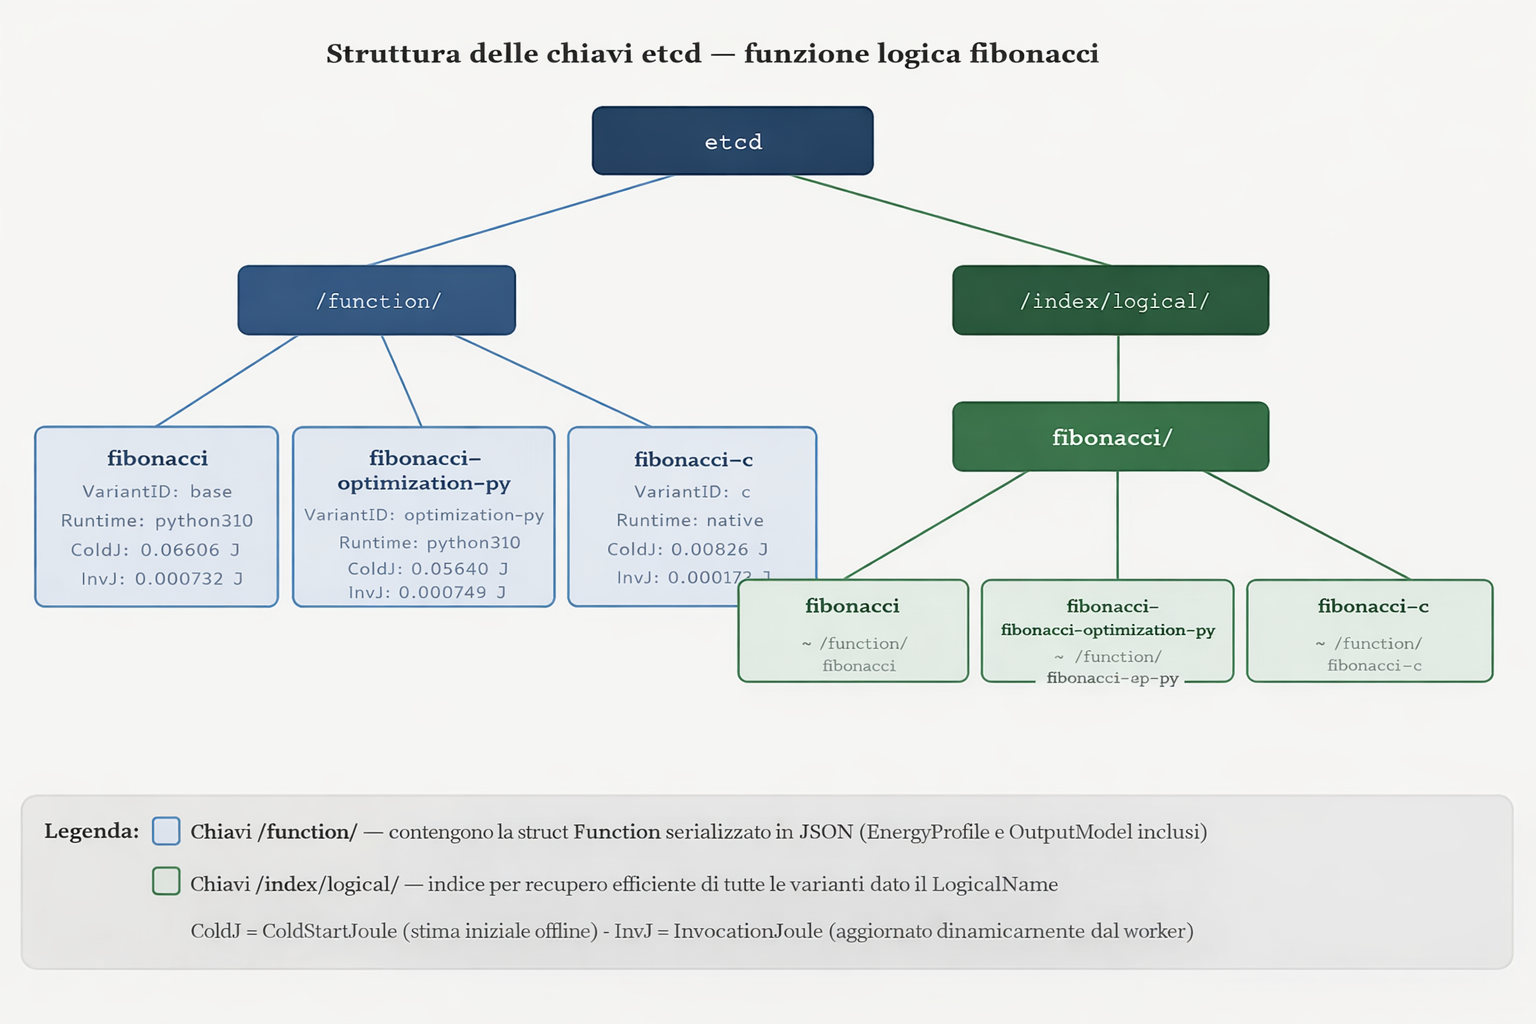
\includegraphics[width=0.95\textwidth]{figures/etcd-structure.jpg}
    \caption{Struttura delle chiavi etcd per la funzione logica 
    \texttt{fibonacci} con tre varianti. Le chiavi sotto 
    \texttt{/function/} contengono i profili completi aggiornati dal 
    worker periodico. L'indice sotto \texttt{/index/logical/} consente 
    allo scheduler di recuperare efficientemente le sole varianti della 
    funzione richiesta, senza scorrere l'intero store.}
    \label{fig:etcd-structure}
\end{figure}